\documentclass[12pt]{article}

\usepackage{tabularx}
\usepackage[a4paper,margin=2.5cm, bottom=2.5cm]{geometry}
\usepackage{fancyhdr}
\usepackage{listings}
\usepackage{booktabs}
\usepackage{float}
\usepackage{subcaption}
% \usepackage{caption}
% \captionsetup{font=footnotesize}
\usepackage{graphicx}
\usepackage{amsmath}
\usepackage{amssymb}
\usepackage{amsthm}
\usepackage{array}
\usepackage[table]{xcolor}
\usepackage{pgfplots}
\pgfplotsset{compat=1.17}
\usepackage{pgfplotstable}
\usepackage{multirow}
\usepackage{tikz}
\usepackage[hidelinks]{hyperref}
\usepackage{titling}
\usepackage[polish]{babel} % Polish language support

\setlength{\headheight}{40pt}
\setlength{\parindent}{0pt}
\setlength{\parskip}{1ex}
\renewcommand{\headrulewidth}{0pt}

\pagestyle{fancy}
\fancyhead{}
\fancyhead[L]{
    \renewcommand{\arraystretch}{1.5}
    \begin{tabularx}{\textwidth}{|X|X|}
        \hline
        \bfseries Obliczenia inteligentne & \bfseries \thetitle \\
        \hline
    \end{tabularx}
}
\fancyfoot[C]{\thepage}

\renewcommand{\maketitle}{
    \thispagestyle{plain}
    \renewcommand{\arraystretch}{2}
    \vspace*{-8em}
    \footnotesize
    \begin{flushleft}
        \begin{tabularx}{\textwidth}{|X|X|}
            \hline
            \bfseries Obliczenia Inteligentne  & \bfseries \thetitle                           \\ \hline
            \multicolumn{2}{|l|}{
                \begin{tabular}[t]{@{}ll@{}} 
                    \textbf{Grupa:} Grupa 1
                    \hspace{4.5em}
                    \textbf{Dzień i czas:} Czwartek, 10:00
                    \hspace{4.5em}
                    \textbf{Rok akademicki:} 2023/24
                \end{tabular}
            } \\ \hline
            \multicolumn{2}{|l|}{
                \begin{tabular}[t]{@{}l@{\hspace{10em}}l@{}} 
                    \textbf{Imię i nazwisko:} \textsc{Jakub Pawlak} & \textbf{Imię i nazwisko:} \textsc{Magdalena Paku\l a} 
                \end{tabular}
            } \\
            \hline
        \end{tabularx}
    \end{flushleft}
    \renewcommand{\arraystretch}{1}
}


\title{Projekt 2 --- Zadanie 1}

\begin{document}
\maketitle
    \section{Opis ekstrakcji cech --- Osoba 1}
    \textbf{Analiza głównych składowych (PCA - Principal Component Analysis)} to technika redukcji wymiarowości danych powszechnie stosowana do ekstrakcji cech. W kontekście zestawu danych MNIST, PCA może być stosowana do zmniejszenia wymiarowości danych obrazowych, zachowując przy tym większość ich wariancji.

    Metoda ekstrakcji cech PCA przekształca dane obrazowe o wysokiej wymiarowości do przestrzeni o niższej wymiarowości, identyfikując główne składowe danych. Te główne składowe to ortogonalne kierunki w przestrzeni cech, które przechwytują maksymalną wariancję danych.

    W naszej implementacji PCA jest stosowana do spłaszczenia każdego obrazu o rozmiarze 28x28 pikseli do wektora o wymiarach 784. Następnie otrzymane wektory są przekształcane do przestrzeni o niższej wymiarowości, zwykle dwóch wymiarów w celu wizualizacji.

    \begin{figure}[h]
        \centering
        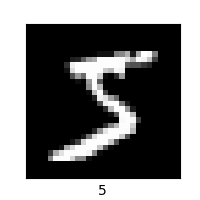
\includegraphics[width=0.3\textwidth]{img/MNIST_1_cyfra}
        \caption{Przykładowy obraz cyfry "5" z zestawu danych MNIST.}
    \end{figure}

    Poniżej znajdują się wygenerowane cechy dla powyższego obrazu "5" za pomocą PCA:
\begin{table}[h]
\centering
\begin{tabular}{|c|c|c|}
\hline
\textbf{Piksel} & \textbf{PCA cecha 1} & \textbf{PCA cecha 2} \\
\hline
1 & -248.0374 & 36.2011 \\
2 & -248.0374 & 36.2011 \\
... & ... & ... \\
28 & -248.0374 & 36.2011 \\
\hline
\end{tabular}
\caption{Wartości wygenerowanych cech za pomocą PCA dla obrazu "5".}
\end{table}



    \textbf{Binary Patterns (LBP)} to deskryptor tekstury używany do ekstrakcji cech w obrazach. W kontekście zestawu danych MNIST, LBP może być stosowany do wydobycia cech tekstury z obrazów.

    Metoda ekstrakcji cech LBP działa przez podzielenie obrazu na małe obszary i porównanie każdego piksela z otaczającymi go pikselami. Na podstawie tych porównań dla każdego piksela tworzony jest wzorzec binarny. Poprzez zliczanie wystąpień różnych wzorców binarnych konstruowany jest histogram reprezentujący cechy tekstury obrazu.

    Poniżej znajdują się wygenerowane cechy dla powyższego obrazu "5" za pomocą LBP:
    \begin{table}[h]
\centering
\begin{tabular}{|c|c|}
\hline
\textbf{LBP cecha} & \textbf{Wartość} \\
\hline
1 & 3.0 \\
2 & 11.0 \\
3 & 6.0 \\
4 & 32.0 \\
5 & 48.0 \\
6 & 34.0 \\
7 & 2.0 \\
8 & 4.0 \\
9 & 618.0 \\
10 & 26.0 \\
\hline
\end{tabular}
\caption{Wartości wygenerowanych cech za pomocą LBP dla obrazu "5".}
\end{table}

    \pagebreak

    \section{Wyniki eksperymentu --- Osoba 1}
    \pagebreak

    \section{Opis ekstrakcji cech --- Osoba 2}
    \textbf{t-Distributed Stochastic Neighbor Embedding (t-SNE) feature extraction:}
    is another dimensionality reduction technique commonly used for visualization. Similar to PCA, t-SNE aims to reduce the dimensionality of the data while preserving its local structure.

    In the context of the MNIST dataset, t-SNE can be applied to reduce the dimensionality of the image data for visualization purposes.

    The t-SNE feature extraction method transforms the high-dimensional image data into a lower-dimensional space, typically two dimensions, while trying to preserve the local structure of the data points.

    \textbf{Histogram of Oriented Gradients (HOG)} is a feature descriptor used for object detection in images. In the context of the MNIST dataset, HOG can be applied to extract shape features from the images.

    The HOG feature extraction method works by calculating the gradient orientation in localized portions of the image. These gradient orientations are then quantized into histogram bins, which are used as features to describe the shape of objects in the image.

    \pagebreak

    \section{Wyniki eksperymentu --- Osoba 2}
    \pagebreak

    \section{Wybór optymalnego modelu}

    Podczas eksperymentów przeprowadzonych w ramach pierwszego projektu dało się zauważyć, że w miarę zwiększania
    liczby neuronów w warstwie ukrytej, skuteczność ewentualnie ulegała wypłaszczeniu.
    W takim przypadku, zwiększanie liczby neuronów skutkowałoby jedynie utrudnieniem obliczeń, bez pozytywnego efektu na skuteczności modelu.
    Optymalnym modelem jest zatem taki, który maksymalizuje dokładność przy jednoczesnym minimalizowaniu ilości neuronów.

    Przeprowadzone eksperymenty nie dostarczyły natomiast jednoznacznego sposobu, aby a priori określić najlepszą liczbę neuronów w warstwie ukrytej.
    Wybór optymalnego modelu został dokonany poprzez coraz dokładnejsze przeszukiwanie przestrzeni liczb naturalnych, podobne w zasadzie działania do algorytmu \emph{binary search}.
    Różne wartości liczby neuronów były poddawane przyśpieszonemu procesowi uczenia (na mniejszym zbiorze danych oraz mniejszą ilością epok), którego to wyniki pozwalały na oszacowanie, które wartości są najbardziej obiecujące.
    Następnie wybierane zostały kolejne ilości neuronów do sprawdzenia --- tym razem z sąsiedztwa najlepiej spisujących się w poprzedniej iteracji.
    Proces powtarzano, aż do znalezienia lokalnego maksimum skutecznośći.

    Metoda ta pozwoliła uzyskać satysfakcjonujące wyniki, jendak wskazać należy, że jesteśmy świadomi iż nie daje ona gwarancji, że wybrany model jest globalnie optymalny.

    \pagebreak

    \section{Wyniki klasyfikacji dla pierwszego sposobu ekstrakcji cech}

    \begin{figure}[H]
        \centering
        \begin{subfigure}[t]{0.3\textwidth}
            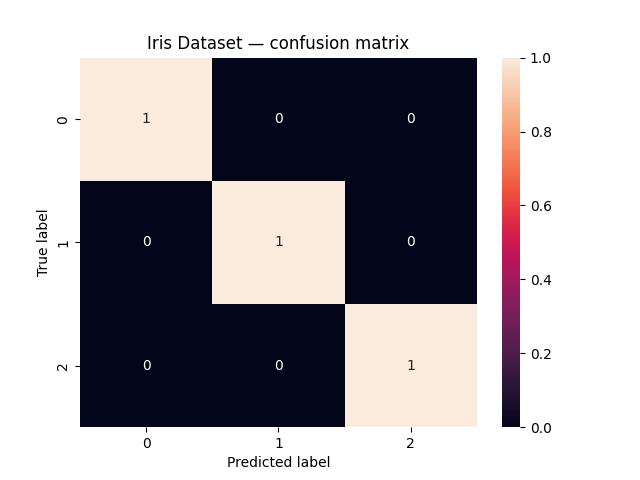
\includegraphics[width=\linewidth]{img/iris_cm.png}
            \caption{Zbior Iris}
        \end{subfigure}
        \hfill
        \begin{subfigure}[t]{0.3\textwidth}
            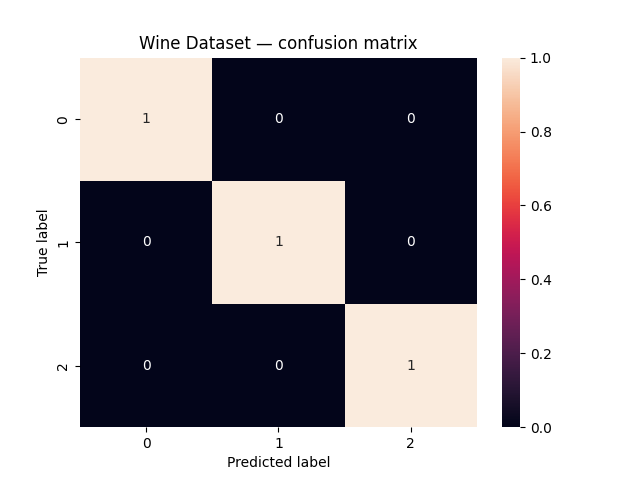
\includegraphics[width=\linewidth]{img/wine_cm.png}
            \caption{Zbior Wine}
        \end{subfigure}
        \hfill
        \begin{subfigure}[t]{0.3\textwidth}
            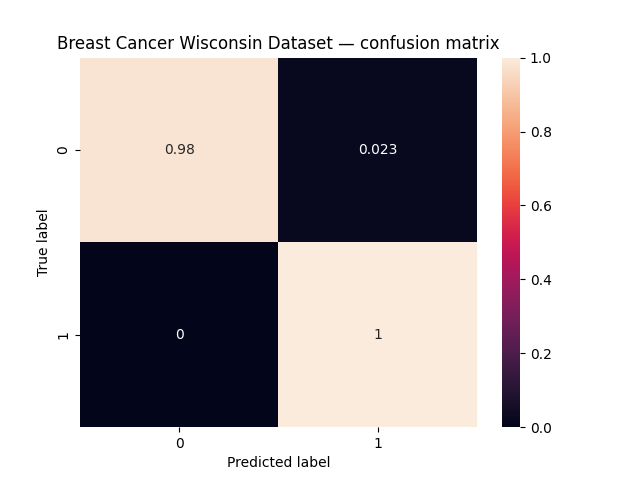
\includegraphics[width=\linewidth]{img/cancer_cm.png}
            \caption{Zbior Breast Cancer Wisconsin}
        \end{subfigure}
        \begin{subfigure}[t]{0.5\textwidth}
            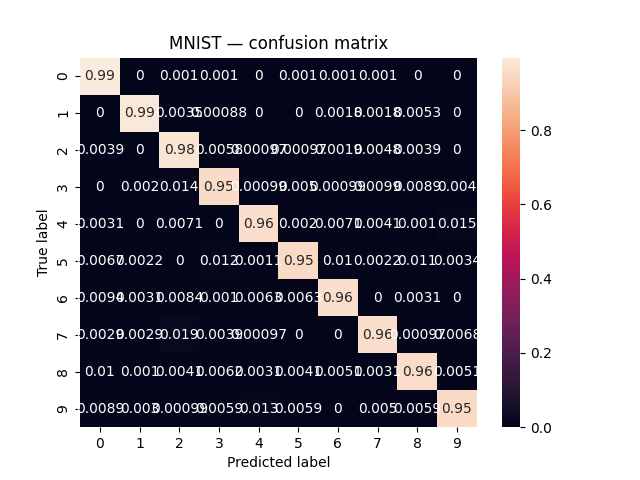
\includegraphics[width=\linewidth]{img/mnist_flat_cm.png}
            \caption{Zbior MNIST}
        \end{subfigure}
        \caption{Wyniki klasyfikacji dla 1 sposobu ekstrakcji cech}
    \end{figure}

    \begin{table}[H]\centering
        \begin{tabular}{lc}
            \toprule
            Zbiór danych & Wartość Accuracy \\
            \midrule
            Iris                    & 93.33\% \\
            Wine                    & 100\% \\
            Breast Cancer Wisconsin & 99.12\% \\
            MNIST                   & 97.16\% \\
            \bottomrule
        \end{tabular}
        \caption{Wartości accuracy wytrenowanego modelu}
    \end{table}

    \pagebreak

    \section{Wyniki klasyfikacji --- Osoba 1}
    \pagebreak

    \section{Wyniki klasyfikacji --- Osoba 2}


    \begin{figure}[H]
        \centering
        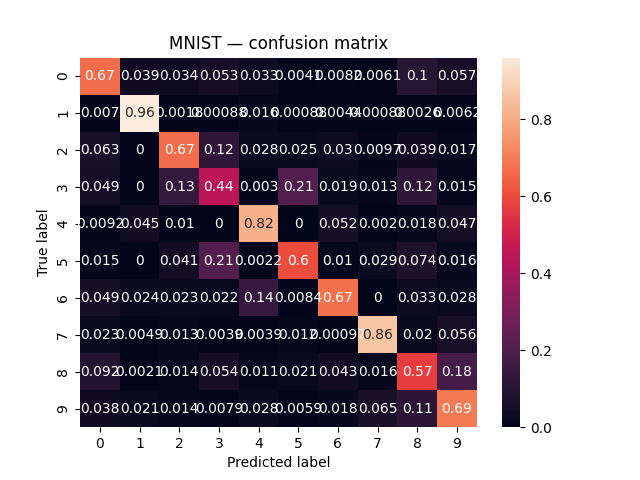
\includegraphics[width=.7\linewidth]{img/mnist_hog_cm.png}
        \caption{Wyniki klasyfikacji dla ekstrakcji cech metodą HOG}
    \end{figure}

    Accuracy: 89.21\%.




\end{document}